\subsection{Posterior Inference under the Extended Model}
Figure~\ref{fig:contour} displays the joint posterior distribution of $(\lambda, A)$, together with the MAP estimate and the corresponding HPD regions. The posterior mode is located at $\lambda \approx 0.0138$ and $A = y_{\max} \approx 179.45$, indicating that the estimate of $A$ coincides exactly with the longest observed tenure in the data. This suggests that the posterior inference of $A$ is strongly driven by the boundary constraint rather than by additional evidence from the data.

First, the posterior distribution of $\lambda$ is highly concentrated, with a relatively narrow range. This shows that the event rate parameter $\lambda$ is primarily determined by the observed event times and can therefore be estimated with high precision. By contrast, the uncertainty associated with $A$ is substantially larger.

Second, the HPD regions exhibit a clear truncation effect at the boundary $A = y_{\max}$. Since the model enforces $A \geq y_{\max}$, the posterior mass is forced against this boundary, creating a sharp cutoff on the left. As a result, the MAP point falls exactly on the boundary, while the 86.5\% HPD region extends almost entirely upward along this edge, forming a one-sided expansion rather than a symmetric spread around the mode, as would be typical under a Gaussian distribution. In other words, the uncertainty in $A$ is essentially about “how much larger than $y_{\max}$ it could be,” rather than about symmetric fluctuations around the MAP.

A closer comparison of the HPD regions further reinforces this interpretation: if the posterior were approximately Gaussian and independent, the 39.3\% and 86.5\% regions would resemble concentric ellipses. In contrast, here the outer region expands asymmetrically in the $A$ direction and clings to the boundary, revealing a boundary-driven skewness rather than Gaussian-like symmetric tails. The slight tilt of the contour also suggests a weak dependence between $\lambda$ and $A$, reflecting the fact that the censoring window and event rate jointly shape the observed data. However, this dependence is secondary compared with the strong boundary effect dominating the inference for $A$.

This observation naturally motivates the marginalization analysis in the next section. By integrating out $A$, we can check whether the extended formulation remains consistent with the baseline exponential model in terms of $\lambda$, thereby clarifying to what extent the introduction of $A$ truly alters—or preserves—the original inferential structure.
\begin{figure}[H]
    \centering
    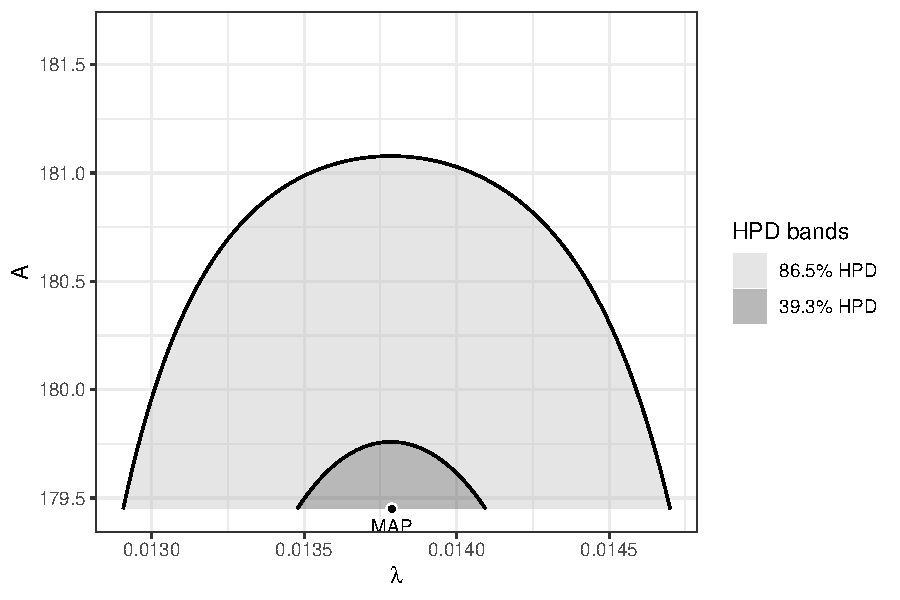
\includegraphics[height=9cm, width=0.65\textwidth]{images/post_contour.pdf}
    \caption{{\small Joint posterior $p(\lambda,A\mid\mathcal D)$ with 39.3\%/86.5\% HPD contours and MAP (black)}}
    \label{fig:contour}
\end{figure}


\subsection{Marginalization and Consistency Check}




\subsection{Baseline Exponential Model Fit}
\label{ecdf的分析}




\subsection{Posterior Predictive Model Checking}